\documentclass[psamsfonts, intlimits, sumlimits, namelimits, 12pt, a4paper]{article}
\usepackage[left = 3.0cm, right = 1.5cm, top = 2.0cm, bottom = 2.0cm]{geometry} % геометрия страницы, в т.ч. поля

\usepackage{caption} % поддержка подписей рисунков и т.д.

\usepackage[T2A]{fontenc} % распознование кодировки текста в tex-файле
\usepackage[utf8]{inputenc}% распознование шрифтов
\usepackage[english, main=russian]{babel}% пакет поддержки орфографий


\usepackage{etex}

% расширенное управление переносом слов, разделенных пунктиром
\usepackage[shortcuts]{extdash}
% поддержка настроек междустрочного интервала
\usepackage{setspace}
% Настройка сносок
\usepackage[perpage,bottom,multiple,stable]{footmisc}

%% Пакеты для гипертекста
\RequirePackage{color}
\usepackage{hyperref} % обширная поддержка гипертекста
\hypersetup{backref,
% colorlinks=false,
linktoc=all
}
\hypersetup{pdfborder=0 0 0}
\hypersetup{pdfencoding=auto}

%% Расширенная математика
\usepackage{amsmath}
\usepackage{amssymb}
\usepackage{amsthm}
\usepackage{amscd}

\usepackage{accents} % пользовательские акценты
\usepackage{cmap} % предоставляет таблицы сопоставления символов для PDF
\usepackage{textcomp} % поддержка шрифтов Text Companion
\usepackage{mathtext} % для "прозрачного" использования кириллических букв в формулах

\usepackage{mathtools}
\mathtoolsset{
showonlyrefs=true, % нумеровать только формулы, на которых есть ссылки
mathic=true,
}

\allowdisplaybreaks

% Поддержка перечислений и списков
\usepackage{paralist}
% \usepackage{enumitem} % не совместим с пакетом paralist
% см. о разнице кратко https://tex.stackexchange.com/questions/18411/what-are-the-differences-between-using-paralist-vs-enumitem

%% Многостраничные таблицы
% \usepackage{longtable}
% \usepackage{lscape}
% \usepackage{makecell}
% \usepackage{multirow}
% \usepackage{tabularx}
% или
\usepackage{tabularray}
\UseTblrLibrary{functional}
\UseTblrLibrary{diagbox}

\DefTblrTemplate{contfoot-text}{russian}{Продолжение на следующей странице}
\SetTblrTemplate{contfoot-text}{russian}
\DefTblrTemplate{conthead-text}{russian}{(Продолжение)}
\SetTblrTemplate{conthead-text}{russian}


%% Работа с графикой
\usepackage{graphicx}

\usepackage{float}
\usepackage{epic}
\usepackage{rotating}

\usepackage[shell, subfolder, cleanup]{gnuplottex}
\def\gnuplotexe{/usr/bin/gnuplot}
% \def\gnuplotexe{C:/Program\ Files/gnuplot/bin/gnuplot.exe}

%% Путь к рисункам
\graphicspath{{images}{gnuplottex}}

%% Обработка текста в eps-файлах
\usepackage[scanall]{psfrag}

%% обработка блок-схем
\usepackage{tikz}
\usetikzlibrary{arrows, shapes, graphs, automata, positioning}

%% Пакеты для библиографии
\usepackage{cite}%
% \usepackage{gost7184}
% \bibliographystyle{gost7184}
% \bibliographystyle{ugost2003s}
\bibliographystyle{gost2008ls}
% \bibliographystyle{utf8gost780u}
%\renewcommand{\bibname}{Литература} % если класс book или report
\renewcommand{\refname}{Литература} % если класс article

%% Пакеты для листингов
%% Расширеное окружение verbatim
\usepackage{fancyvrb}
\usepackage{url}

% Наряду, или вместо verbatim можно использовать более специализированный.
% Пакет listings
\usepackage{listings}
\usepackage{listingsutf8}
\lstset{%
    showstringspaces=false,
    numbers=left,
%    numberstyle=\tiny,
%    upquote=false,
    keepspaces=true,
    columns=flexible,
    basicstyle=\footnotesize\ttfamily,%
    breaklines=true,%
    breakatwhitespace=true,%
    postbreak=\space,%
    prebreak={\mbox{\quad$\hookleftarrow$}},%
}

%\ifthenelse{\boolean{luatex}\OR\boolean{xetex}}{}{%
%    \lstset{inputencoding=utf8/koi8-r}}

\lstloadlanguages{C,make,bash,[x86masm]Assembler,[LaTeX]TeX, [08]Fortran, [95]Fortran, Gnuplot}

\usepackage{indentfirst} % отступ первой строки каждого раздела по умолчанию
% \renewcommand\baselinestretch{1} % междустроный интервал всего документа

\ifx\pstmode\undefined
\else
    \setbeamertemplate{navigation symbols}{}
\fi

\ifdefined\withnotes
	\usepackage{pgfpages}

	\ifdefined\onlynotes
	\setbeameroption{show only notes}
	\setbeamertemplate{note page}[compress]
	\pgfpagesuselayout{resize to}[a4paper,border shrink=5mm,landscape]
	\else
	\setbeameroption{show notes}
	\setbeamertemplate{note page}[plain]
	\pgfpagesuselayout{8 on 1}[a4paper,border shrink=5mm]
	\fi

	% Версия для печати
	\ifdefined\printable
	  \usecolortheme{dove}
	  \setbeamertemplate{navigation symbols}{}
	  \setbeamercolor{note page}{bg=white}
	  \setbeamercolor{note title}{bg=white}
	  \setbeamercolor{note date}{bg=white}
	\fi

	% http://tex.stackexchange.com/questions/288408/beamer-show-notes-on-second-screen-with-xelatex-and-atbeginsection
	\ifthenelse{\boolean{xetex}}{%
	  \makeatletter
	  \def\beamer@framenotesbegin{% at beginning of slide
		 \usebeamercolor[fg]{normal text}
		 \gdef\beamer@noteitems{}%
		 \gdef\beamer@notes{}%
	  }
	  \makeatother
	}{}
\else\fi

\ifdefined\handoutwithnotes
	\usepackage{handoutWithNotes}
	\pgfpagesuselayout{4 on 1 with notes}[a4paper,border shrink=5mm]
\else\fi

\ifdefined\poster
	\mode<presentation> {
		 \usetheme{PFU}				% Название темы оформления для постера
		 \setbeamertemplate{navigation symbols}{}	% Убираем навигационные символы
	}

	\usepackage{ragged2e}
	\boldmath			% Математические формулы будут полужирными, чтоб в глаза било

	%\usepackage[orientation=album,size=a0,scale=1.4,debug]{beamerposter}                       	% e.g. for DIN-A0 poster
	%\usepackage[orientation=portrait,size=a1,scale=1.4,grid,debug]{beamerposter}                  	% e.g. for DIN-A1 poster, with optional grid and debug output
	%\usepackage[size=custom,width=200,height=120,scale=2,debug]{beamerposter}                     	% e.g. for custom size poster
	%\usepackage[orientation=portrait,size=a0,scale=1.0,printer=rwth-glossy-uv.df]{beamerposter}   	% e.g. for DIN-A0 poster with rwth-glossy-uv printer check
	%\usepackage[orientation=album,size=a0,scale=1.4]{beamerposter}
	\usepackage[orientation=portrait,size=a1,scale=1.0]{beamerposter}
\else\fi

\usepackage{pifont}

%% настройки геометрии
%\RequirePackage{xkeyval}

\usepackage{bm} % определяет команду \bm{<текст>} дающее полужирное начертание тексту <текст> в аргументе

\usepackage{texnames}

\usepackage{wrapfig} % позволяет обернуть текст вокруг рисунков или таблиц

\def\bibnamefont{\textit} % задаёт курсив Ф.И.О. авторов в списке литературы

\usepackage{calc}
\usepackage{soulutf8} % пакет soul с поддержкой utf8: позволяет быстро форматировать текст, например выделить командой \hl


% \usepackage[nodayofweek]{datetime}
\usepackage[24hr]{datetime}

\nocite{*} %  включает в спиcок литературы все записи что без ссылок в тектсе через \cite

\usepackage{afterpage}
\usepackage{subfigure}
\renewcommand{\thesubfigure}{\asbuk{subfigure}}

\begin{document}

% титульная часть

\title{%
	\Large\bfseries
	Краткое введение в \LaTeX \\
	и основы работы с Gnuplot
}

\author{\large\bfseries Ниеолаев~Н.~Э.$^{1,2)}$,  Гоним~Н.$^{1,3)}$} %

\date{%
	\normalsize\itshape
	$^{1)}$Институт физических исследований и технологий \\
	Российский университет дружбы народов \\
	Россия, 117198, Москва, ул. Миклухо-Маклая, 6 \\[1ex]
	$^{2)}$nikolaev\_\!ne@pfur.ru, $^{3)}$gonim\_\!m@pfur.ru
}

\maketitle

%% Аннотация

{\small\indent Рассматриваются некоторые возможности языка программирования \LaTeX\ для подготовки отчётов, научных статей и др. Приводятся примеры с небольшим пояснением, в том числе работа с математическими формулами, графиками, таблицами, листингом и блок\nobreak-схемами.
}\\[1ex]

\indent {\bfseries Ключевые слова:} издательская система, язык программирования, построение графиков, построение таблиц, построение блок\nobreak-схем, \LaTeX, листинг, оформление математических выражений.



% введение
\section{Введение}
\label{sec:introduction}


\LaTeX\ "--- научная издательская система, в первую очередь предназначенная для подготовки научных публикаций, что выражается в наличии развитого аппарата для быстрого набора математических выражений, диаграмм, физических и химических формул, средств внедрения в текст графических файлов~\cite{nasyrov:book:2019:01}.

В \LaTeX\ очень удобно реализован процесс нумерации объектов: формул, рисунков, таблиц, литературы и т.д., основанный на использовании уникальных меток, присваиваемых пользователем соответствующим объектам. Эта особенность системы особенно ценится пользователями системы, так как добавление или удаление в тексте документа объекта, нарушающего сквозную нумерацию, например, формулы, не требует ручной корректировки нумерации по всему документу, всю рутинную работу \LaTeX\ выполнит автоматически в процессе компиляции окончательного файла документа.

Ещё одно существенное преимущество \LaTeX\ "--- это особая структура документа, позволяющая пользователю иметь уверенность, что при наборе текста и последующем редактировании не собьется форматирование: формулы, рисунки, таблицы и фрагменты текста останутся такими же и в тех жеместах документа. Эту особенность используют редакции серьёзных научных изданий, широко применяя \LaTeX\ при верстке журналов, когда к статьям,набранным разными авторами, применяется одинаковый набор стилевых инструкций, автоматически приводящий эти статьи к единому оформлению.

Как издательская система \LaTeX\ представляет собой набор компьютерных программ (пакетов), однако с точки зрения конечного пользователя этой системы \LaTeX\ "--- это свод правил и команд, по которым исходный текст документа преобразуется в окончательную печатную версию, в этом смысле \LaTeX\ "--- это язык программирования, которым пользователь системы должен владеть. Первую версию \LaTeX\ создал Лесли Лэмпорт, который в 1985 г. представил набор макросов (макрокоманд) как надстройку над системой подготовки печатной документации \TeX, разработанной Дональдом Кнутомв 1979 г. Система команд \TeX\ фактически была первым языком разметки гипертекста, а её исполняемая программа "--- <<tex.exe>>, выполнявшая преобразование размеченного текста в документ, пригодный для печати, была одной из первых программ парсеров (parser). Первый перевод~\cite{knut:book:1993:01} классической книги Дональда Кнута <<The \TeX\ book>>~\cite{knut:book:1984:01} c наиболее полной информацией об этой системе, опубликован в России в 1993 г.

Язык \TeX\ относится к языкам программирования низкого уровня и достаточно сложен в использовании, поэтому, несмотря на то, что \TeX\ до сих пор общепризнанно является наиболее качественной системой подготовки научных печатных публикаций, <<чистый>> \TeX\ сейчас используется главным образом при разработке классов и пакетов для \LaTeX.



% раздел 1
\section{Начало работы}
\label{sec:nachalo_raboty}


Для начала следует установить \TeX-систему, настоятельно рекомендуется поставить \texttt{texlive} (есть на трёх платформах \textit{linux, windows, mac},~см.~\url{https://tug.org/texlive}), представляющий собой самый полный набор tex\nobreak-программ\footnote{В отличии от \texttt{miktex}, \textbf{не рекомендуется} ставить последний, как например в~\cite{nasyrov:book:2019:01}} и возможности настройки.

Исходный код представляет собой текст набранный, как упоминалось, на специальном языке, сохраннёный в обычном тектовом файле с расширением <<tex>>, например \texttt{default.tex}

Для того чтобы скомпилировать tex\nobreak-файл, необходимо вызвать в консоли (терминале, командной строке) программу \texttt{pdflatex} и передать в качестве параметра имя файла (расширение указывать необязательно), также рекомендуется включать режим синхронизации с исходным кодом ключом \texttt{synctex}. Тогда \verb|pdflatex --synctex=1 default|.

Любой \LaTeX овский (или \TeX овский) документ состоит из двух частей: из преамбулы (\texttt{preambule}) и тела документа (заключённого в окружении \texttt{document}). Вся стилистика, то есть правила форматирования тела документа задаются набором команд из которых и образована преамбула документа. Например для начала работы с мультиязычным вводом (русский и английский), вводом математических формул и вставки графики достаточно в преамбуде подключить всего несколько пакетов:
\begin{Verbatim}[frame = single, label = {Пример tex\nobreak-файла \LaTeXовского документа}, fontfamily = courier, tabsize = 3, numbers = left, gobble=1]
	% преамбула документа
	\documentclass[12pt,a4paper]{article}
	\usepackage[left=3.0cm, right=1.5cm, top=2.0cm,
		bottom=2.0cm]{geometry}	% геометрия страницы, в т.ч. поля
	\usepackage[utf8]{inputenc}	% распознование кодировки текста в tex-файле
	\usepackage[T2A]{fontenc} % распознование шрифтов
	\usepackage[english, main=russian]{babel}	% пакет поддержки орфографий
	\usepackage{amsmath,amsfonts,amssymb} % пакеты ввода матформул
	\usepackage{graphicx}% пакеты поддержки вставки рисунков

	\begin{document}
		% тело документа
		{\selectlanguage{russian}
		Здесь может будь ваш собственный текст.
		} % END \selectlanguage

		{\selectlanguage{english}
		Your own text can be here.
		} % END \selectlanguage
	\end{document}
\end{Verbatim}
Преамбула всегда начинается командой:

\verb|\documentclass[<параметры_класса_документа>]{<имя_класса_документа>}|;

\noindent однако рекомендуется использовать преамбулу в искодном tex\nobreak-файле данного документа, при этом подключаемый файл \texttt{define.tex} командой \textsc{include}: \verb|\ifx\pstmode\undefined
\else
    \setbeamertemplate{navigation symbols}{}
\fi

\ifdefined\withnotes
	\usepackage{pgfpages}

	\ifdefined\onlynotes
	\setbeameroption{show only notes}
	\setbeamertemplate{note page}[compress]
	\pgfpagesuselayout{resize to}[a4paper,border shrink=5mm,landscape]
	\else
	\setbeameroption{show notes}
	\setbeamertemplate{note page}[plain]
	\pgfpagesuselayout{8 on 1}[a4paper,border shrink=5mm]
	\fi

	% Версия для печати
	\ifdefined\printable
	  \usecolortheme{dove}
	  \setbeamertemplate{navigation symbols}{}
	  \setbeamercolor{note page}{bg=white}
	  \setbeamercolor{note title}{bg=white}
	  \setbeamercolor{note date}{bg=white}
	\fi

	% http://tex.stackexchange.com/questions/288408/beamer-show-notes-on-second-screen-with-xelatex-and-atbeginsection
	\ifthenelse{\boolean{xetex}}{%
	  \makeatletter
	  \def\beamer@framenotesbegin{% at beginning of slide
		 \usebeamercolor[fg]{normal text}
		 \gdef\beamer@noteitems{}%
		 \gdef\beamer@notes{}%
	  }
	  \makeatother
	}{}
\else\fi

\ifdefined\handoutwithnotes
	\usepackage{handoutWithNotes}
	\pgfpagesuselayout{4 on 1 with notes}[a4paper,border shrink=5mm]
\else\fi

\ifdefined\poster
	\mode<presentation> {
		 \usetheme{PFU}				% Название темы оформления для постера
		 \setbeamertemplate{navigation symbols}{}	% Убираем навигационные символы
	}

	\usepackage{ragged2e}
	\boldmath			% Математические формулы будут полужирными, чтоб в глаза било

	%\usepackage[orientation=album,size=a0,scale=1.4,debug]{beamerposter}                       	% e.g. for DIN-A0 poster
	%\usepackage[orientation=portrait,size=a1,scale=1.4,grid,debug]{beamerposter}                  	% e.g. for DIN-A1 poster, with optional grid and debug output
	%\usepackage[size=custom,width=200,height=120,scale=2,debug]{beamerposter}                     	% e.g. for custom size poster
	%\usepackage[orientation=portrait,size=a0,scale=1.0,printer=rwth-glossy-uv.df]{beamerposter}   	% e.g. for DIN-A0 poster with rwth-glossy-uv printer check
	%\usepackage[orientation=album,size=a0,scale=1.4]{beamerposter}
	\usepackage[orientation=portrait,size=a1,scale=1.0]{beamerposter}
\else\fi

\usepackage{pifont}

%% настройки геометрии
%\RequirePackage{xkeyval}

\usepackage{bm} % определяет команду \bm{<текст>} дающее полужирное начертание тексту <текст> в аргументе

\usepackage{texnames}

\usepackage{wrapfig} % позволяет обернуть текст вокруг рисунков или таблиц

\def\bibnamefont{\textit} % задаёт курсив Ф.И.О. авторов в списке литературы

\usepackage{calc}
\usepackage{soulutf8} % пакет soul с поддержкой utf8: позволяет быстро форматировать текст, например выделить командой \hl


% \usepackage[nodayofweek]{datetime}
\usepackage[24hr]{datetime}

\nocite{*} %  включает в спиcок литературы все записи что без ссылок в тектсе через \cite

\usepackage{afterpage}
\usepackage{subfigure}
\renewcommand{\thesubfigure}{\asbuk{subfigure}}|; необязателен.

Отметим, что фигурные скобки \textsc{\{ \}} у команд отвечают за обязательные параметры, квадратные \textsc{[ ]} "--- за необязательные. Например, любое окружение в \LaTeX\ вводится командами \textsc{begin} и \textsc{end}: \verb|\begin{<имя_окружения>}| \ldots \verb|\end{<имя_окружения>}|.
Фигурные скобки используются также для выделения объекта, например,для указаные области действия некоторых команд; допустим, используя команду \textsc{bfseries} или \textsc{itshape} чтобы изменить начернатие текста на {\bfseries полужирное} или {\itshape курсивное} соответствено, впишем их внутри фигурных скобок, тогда действие этих команд будет ограничено в пределах данных скобок: \verb|{\bfseries полужирный текст}|, \verb|{\itshape курсивный текст}|. Важно помнить, что язык \TeX\ "--- регистрозависимый.

Подробнее введение в \LaTeX\ см.~в~\cite{nasyrov:book:2019:01}.

% раздел 2
\section{Ввод формул и их нумерация}
\label{sec:vvod_formul_i_ix_numeraciya}


Допустим, мы хотим ввести уравнения Максвелла в переменных Майорана \\ $\xi = E + i H$ и $\eta = E - i H$ для электромагнитного поля вне источников. Обратим внимание что строчные формулы для переменных $\xi$ и $\eta$ вводятся в {\itshape математической моде}, для входа в которую используется символ \$ (доллара). Для выхода из неё, возвращаясь в {\itshape текстовую моду}, повторно вводится символ \$. Уравнения же введём в виде <<формулы-выключки>> (на выделенной строке), используя окружение \textsc{equation}:

\hl{Источник:}

\begin{Verbatim}[frame = single, label = {Пример окружения \textsc{equation}}, fontfamily = courier, tabsize = 3, numbers = left, gobble=1]
	\begin{equation}
		\label{eq:uravneniya_maksvella_v_peremennyx_majorana}
		\begin{cases}
			\frac{\partial}{\partial t} \xi = (s,\nabla) \xi , & \operatorname{div} \xi = 0 , \\
			\frac{\partial}{\partial t} \eta = (s,\nabla) \eta , & \operatorname{div} \eta = 0 ,
		\end{cases}
	\end{equation}
\end{Verbatim}

\hl{Вывод:}

\begin{equation}
	\label{eq:uravneniya_maksvella_v_peremennyx_majorana}
	\begin{cases}
		\frac{\partial}{\partial t} \xi = (s,\nabla) \xi , & \operatorname{div} \xi = 0 , \\
		\frac{\partial}{\partial t} \eta = (s,\nabla) \eta , & \operatorname{div} \eta = 0 ,
	\end{cases}
\end{equation}
где $s$ - оператор спина фотона~(см.~\cite{axiezer:book:1981:01}), представляющий собой вектор-матрицу со слагающими $s_{j} = i A_{j}$ $\forall j =\overline{1,3}$. Здесь $A_{j}$ "--- матрицы бесконечно малых поворотов вокруг соответствующих осей трёхмерного евклидового пространства~\cite{gelfand:book:1972:09}.

Нумерация формул автоматическая, и согласно установке в преамбуле, нумеруются те формулы на которые есть хотя бы одна ссылка в тексте. Прежде нам необходимо установить \textit{уникальную метку} через команду \textsc{label} в качестве её аргумента. Далее чтобы сослаться на метку достаточно воспользоваться командой \textsc{ref}, но поскольку мы хотим сослаться на формулу, воспользуемся специально отведённой для этого командой \textsc{eqref}. Для уравнений выше мы напишем:

\verb|\eqref{eq:uravneniya_maksvella_v_peremennyx_majorana}|,

\noindent где "eq" обозначает то что мы ссылаемся на объект окружения \textsc{equation}, затем следует имя метки после ":". Рекомендуется следовать этому регламенту. Разница между командами \textsc{ref} и \textsc{eqref} состоит в том что последняя выводить метку (номер) в круглых скобках. Так отметим что выражения справа в~\eqref{eq:uravneniya_maksvella_v_peremennyx_majorana} представляют собой специальные условия на дивергенцию решений уравнений Максвелла.

Отметим что <<формулы-выключки>> можно также ввести заключив между "\verb|\[|" и "\verb|\]|", но нумеровать такие формулы невозможно с помощью команды \textsc{label}, при этом в \LaTeX\ сохраняется \TeX овский вариант ввода таких формул, а именно заключив описание формулы между "\$\$"\ и "\$\$".



% раздел 4
\section{Работа с таблицами и листингом}
\label{sec:rabota_s_tablicami_i_listingom}

Нам необходимо ввести и оформить таблицу. Для этого можно подключать совокупность пакетов (см.~преамбулу данного документа) по необходимости, однако мы здесь рассмотрим один мощный пакет \textsc{tabularray}, например, мы хотим оформить большую таблицу на несколько страниц следующим образом:

\hl{Источник:}

%\lstset{language = [LaTeX]TeX, inputencoding = utf8, frame = none, tabsize = 3, numbers = left, numbersep = 6pt, gobble=1}%
%\begin{lstlisting}
\begin{Verbatim}[frame = single, label = {Пример окружения \textsc{longtblr}}, fontfamily = courier, tabsize = 3, numbers = left, gobble=1]
	\begin{longtblr}[
	% 	theme = fancy,
		caption = {Большая таблица, но на самом деле короткая.},
		entry = {Большая короткая таблица},
		label = {tblr:bolshaya_tablica_no_na_samom_dele_korotkaya},
		note{a} = {Это первая сноска.},
		note{$\dag$} = {Это вторая длинная сноска.},
		remark{Примечание} = {Некоторые общие примечания.},
		remark{Источник} = {Сделано силами авторов.},
	]{
		colspec = {|l|l|l|},
		row{odd} = {bg = azure8},
		row{1} = {c, bg = azure3, fg = white, font = \sffamily},
		rowhead = 1,
		rowfoot = 0,
	}
		\hline
		$\alpha$ & $\beta$ & $\gamma$ \\
		\hline
		$\delta$ & $\epsilon$ & $\zeta$ \\
		\hline
		$\eta$ & $\theta$ & $\iota$ \\
		\hline
		$\kappa$ & $\lambda$ & $\mu$ \\
		\hline
		$\nu$ $\xi$ $o$ & $\pi$ $\rho$ $\sigma$ & $\tau$ $\upsilon$ $\phi$ \\
		\hline
	\end{longtblr}
\end{Verbatim}

\newpage

\hl{Вывод:}

\begin{longtblr}[
% 	theme = fancy,
	caption = {Большая таблица, но на самом деле короткая.},
	entry = {Большая короткая таблица},
	label = {tblr:bolshaya_tablica_no_na_samom_dele_korotkaya},
	note{a} = {Это первая сноска.},
	note{$\dag$} = {Это вторая длинная сноска.},
	remark{Примечание} = {Некоторые общие примечания.},
	remark{Источник} = {Сделано силами авторов.},
	baseline = m,
]{
	colspec = {|l|l|l|},
	row{odd} = {bg = azure8},
	row{1} = {c, bg = azure3, fg = white, font = \sffamily},
	rowhead = 1,
	rowfoot = 0,
}
	\hline
	$\alpha$ & $\beta$ & $\gamma$ \\
	\hline
	$\delta$ & $\epsilon$ & $\zeta$ \\
	\hline
	$\eta$ & $\theta$ & $\iota$ \\
	\hline
	$\kappa$ & $\lambda$ & $\mu$ \\
	\hline
	$\nu$ $\xi$ $o$ & $\pi$ $\rho$ $\sigma$ & $\tau$ $\upsilon$ $\phi$ \\
	\hline
\end{longtblr}

Здесь мы воспользовались окружением \textsc{longtblr}, если же наша таблица помещается на одной странице, то достаточно использовать окружение \textsc{tblr}. Заметьте, что метку \texttt{label} мы указали в необязательных параметрах (т.е. в \textsc{[ ]} скобках), а не в теле окружения, как это сделано в окружении \textsc{equation}. Пример результата вывода многостраничной таблицы см.~в~прил.

Для листинга программы воспользуемся окурением \textsc{verbatim}, например подключив пакет \textsc{fancyvrb}. В необязательных параметрах окружения \textsc{Verbatim} выберем шрифт \texttt{courier}, размер табуляции равным трём, а номера строк расположим слева:
{
\begin{verbatim}
	\begin{Verbatim}[fontfamily = courier, tabsize = 3, numbers = left, gobble=1]
	...
	\end{Verbatim}%
\end{verbatim}
}
В теле окружения прописываем текст исходного кода программы, кроме того можно непосредственно подключать сам файл исходного кода, воспользовавшись командой \textsc{VerbatimInput}, например: \verb|\VerbatimInput[fontfamily=courier, tabsize=3,|\\ \verb|numbers=left, numbersep=6pt]{src/testx3p.f08}|. Данный пакет хоть и прост в освоении, всё же довольно грубо приводит листинг. Для этих целей лучше подходит пакет \textsc{listings}, более специализированный. Им и воспользуемся для оистинга программы далее.



% раздел 4
\section{Работа с графикой и блок\nobreak-схемами}
\label{sec:rabota_s_grafikoj_i_blok_sxemami}


Рассмотрим вставку готового рисунка. Для этого воспользуемся командой\\ \textsc{includegraphics} из пакета \textsc{graphicx}, но поскольку нам необходимо ещё подпись к нему и возможность сослаться, то ещё воспользуемся окружением \textsc{figure}.
{
%\lstset{language = [LaTeX]TeX, inputencoding = utf8, frame = none, tabsize = 3, numbers = left, numbersep = 6pt, gobble=1}%
%\begin{lstlisting}
\begin{Verbatim}[fontfamily = courier, tabsize = 3, numbers = left, gobble=1]
	\begin{figure}[H]
		\center{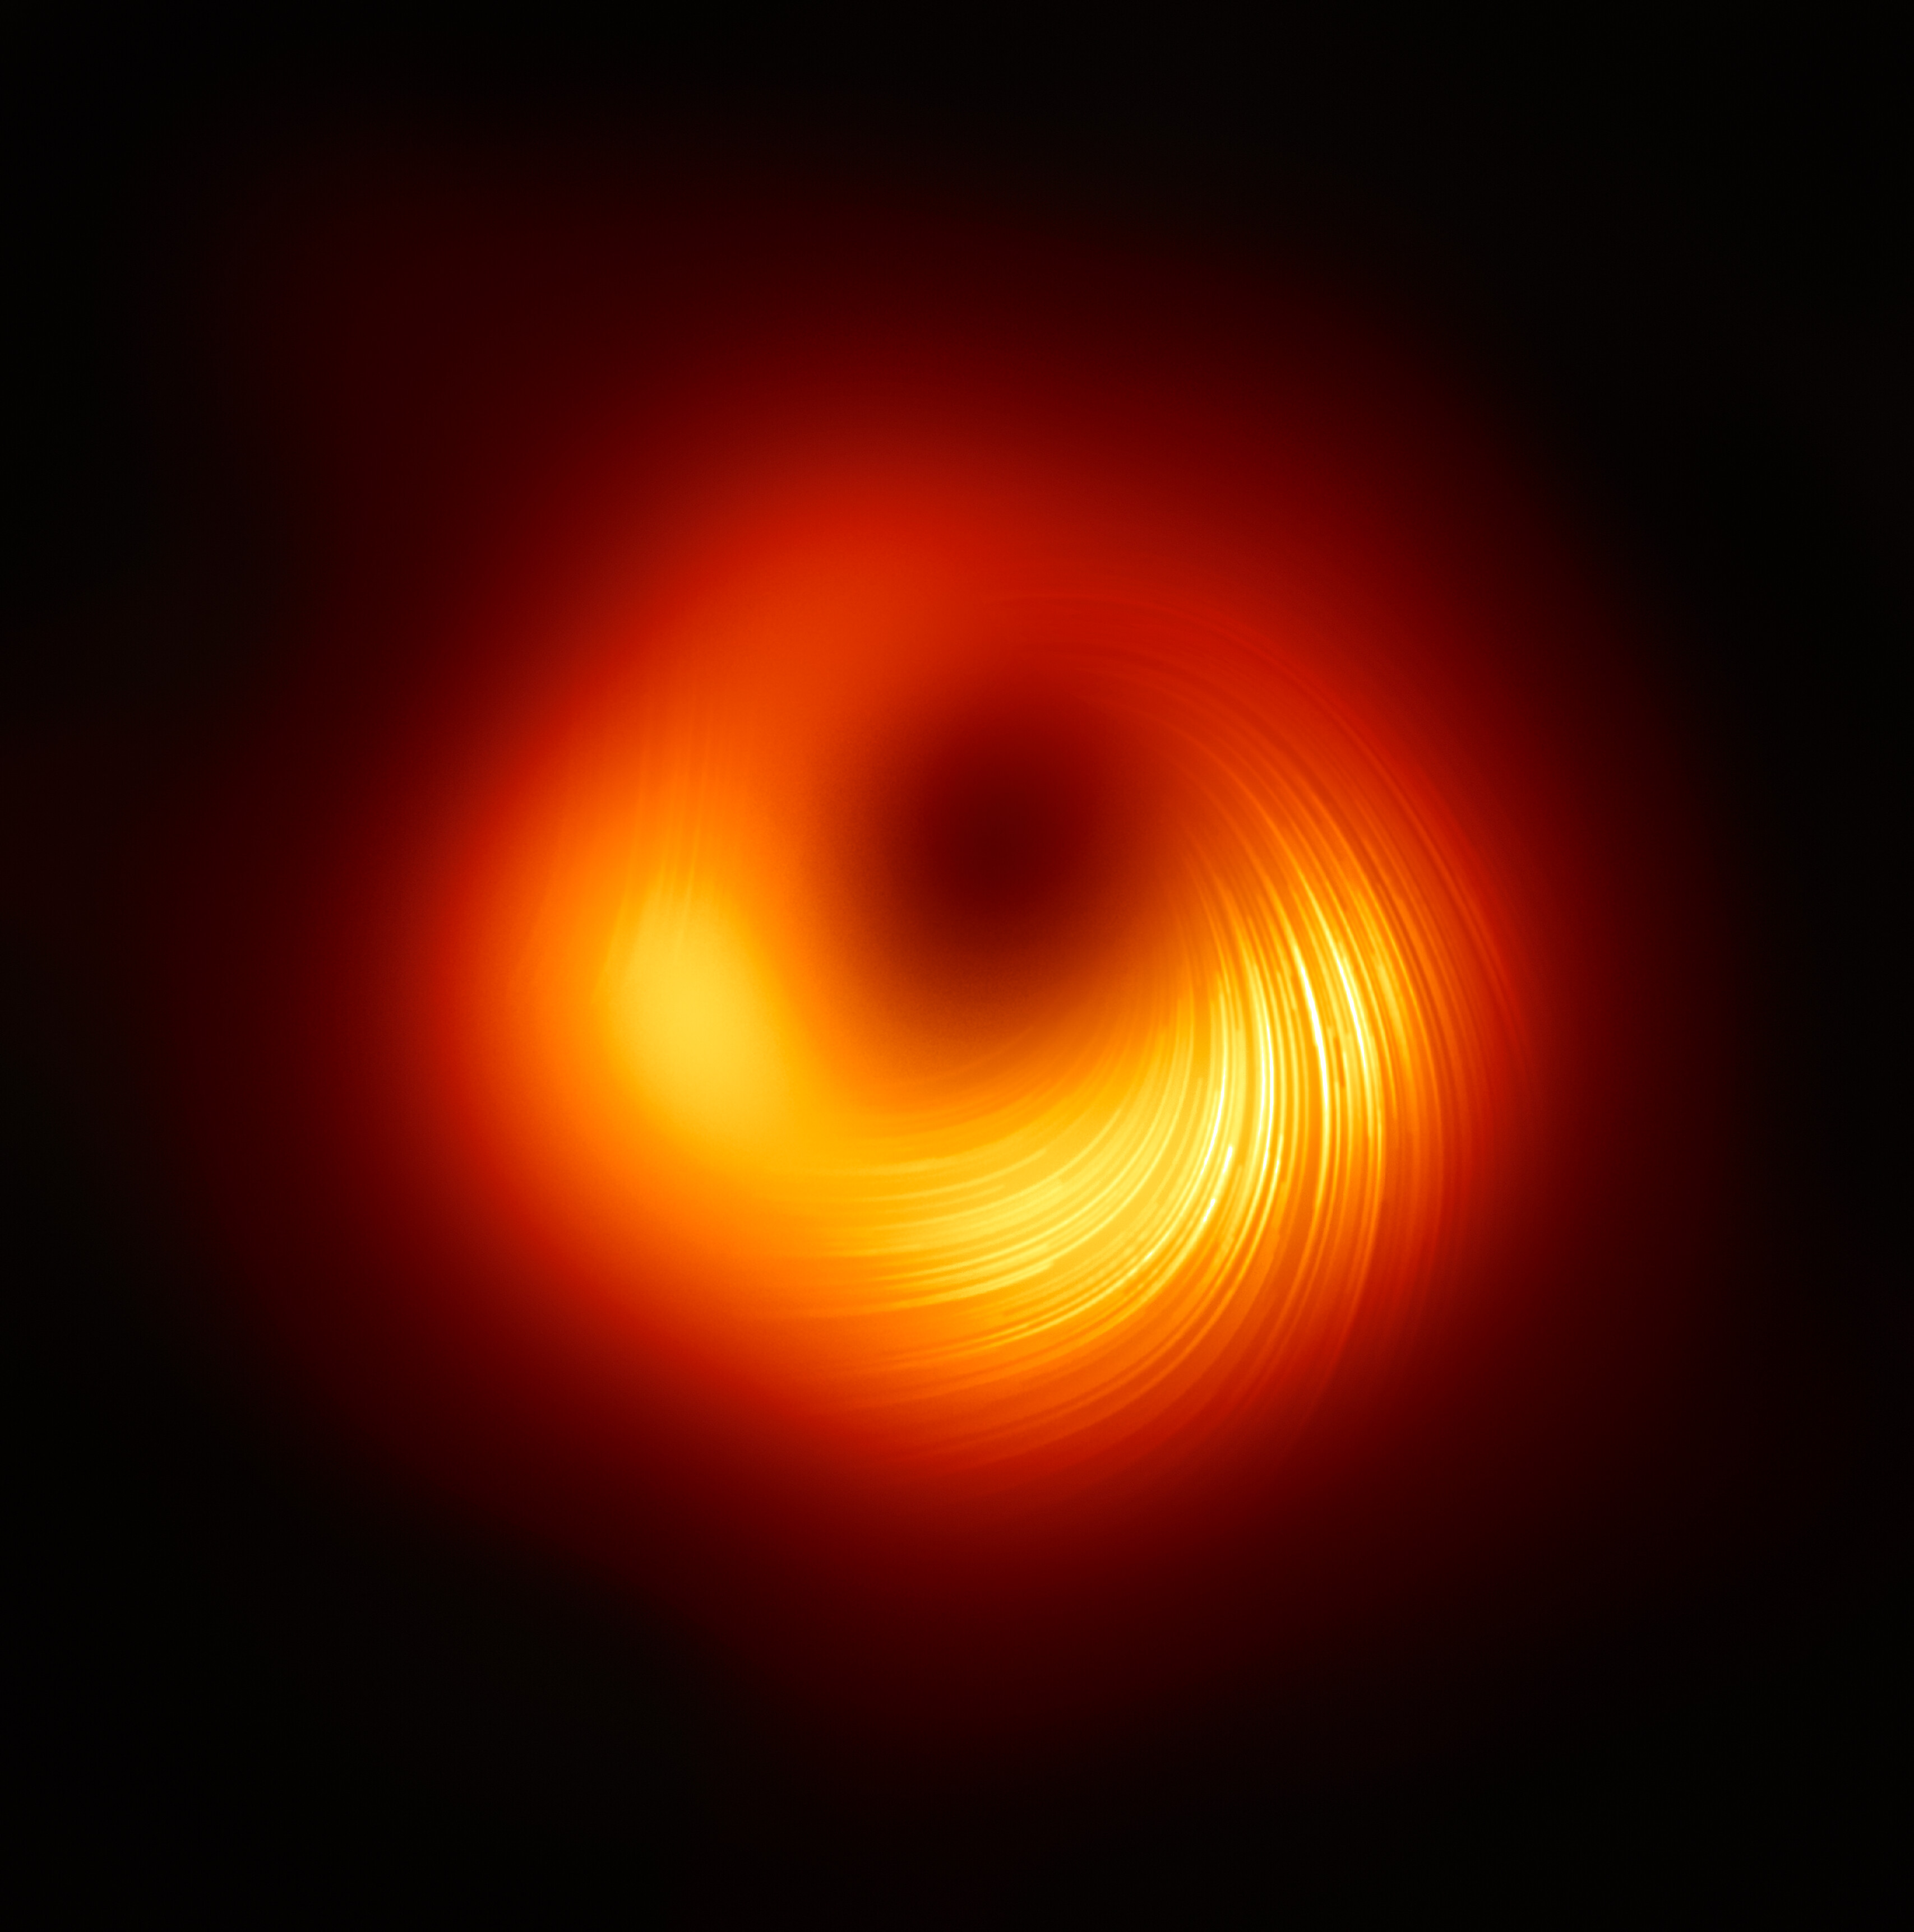
\includegraphics[width=0.7\linewidth]{c96e01c894dab21d52bb0bd6565f0331.jpg}}
		\caption{Восстановленная фотография тени чёрной дыры.}
		\label{fig:vosstanovlennaya_fotografiya_chyornoj_dyry}
	\end{figure}
\end{Verbatim}
}
\begin{figure}[H]
	\center{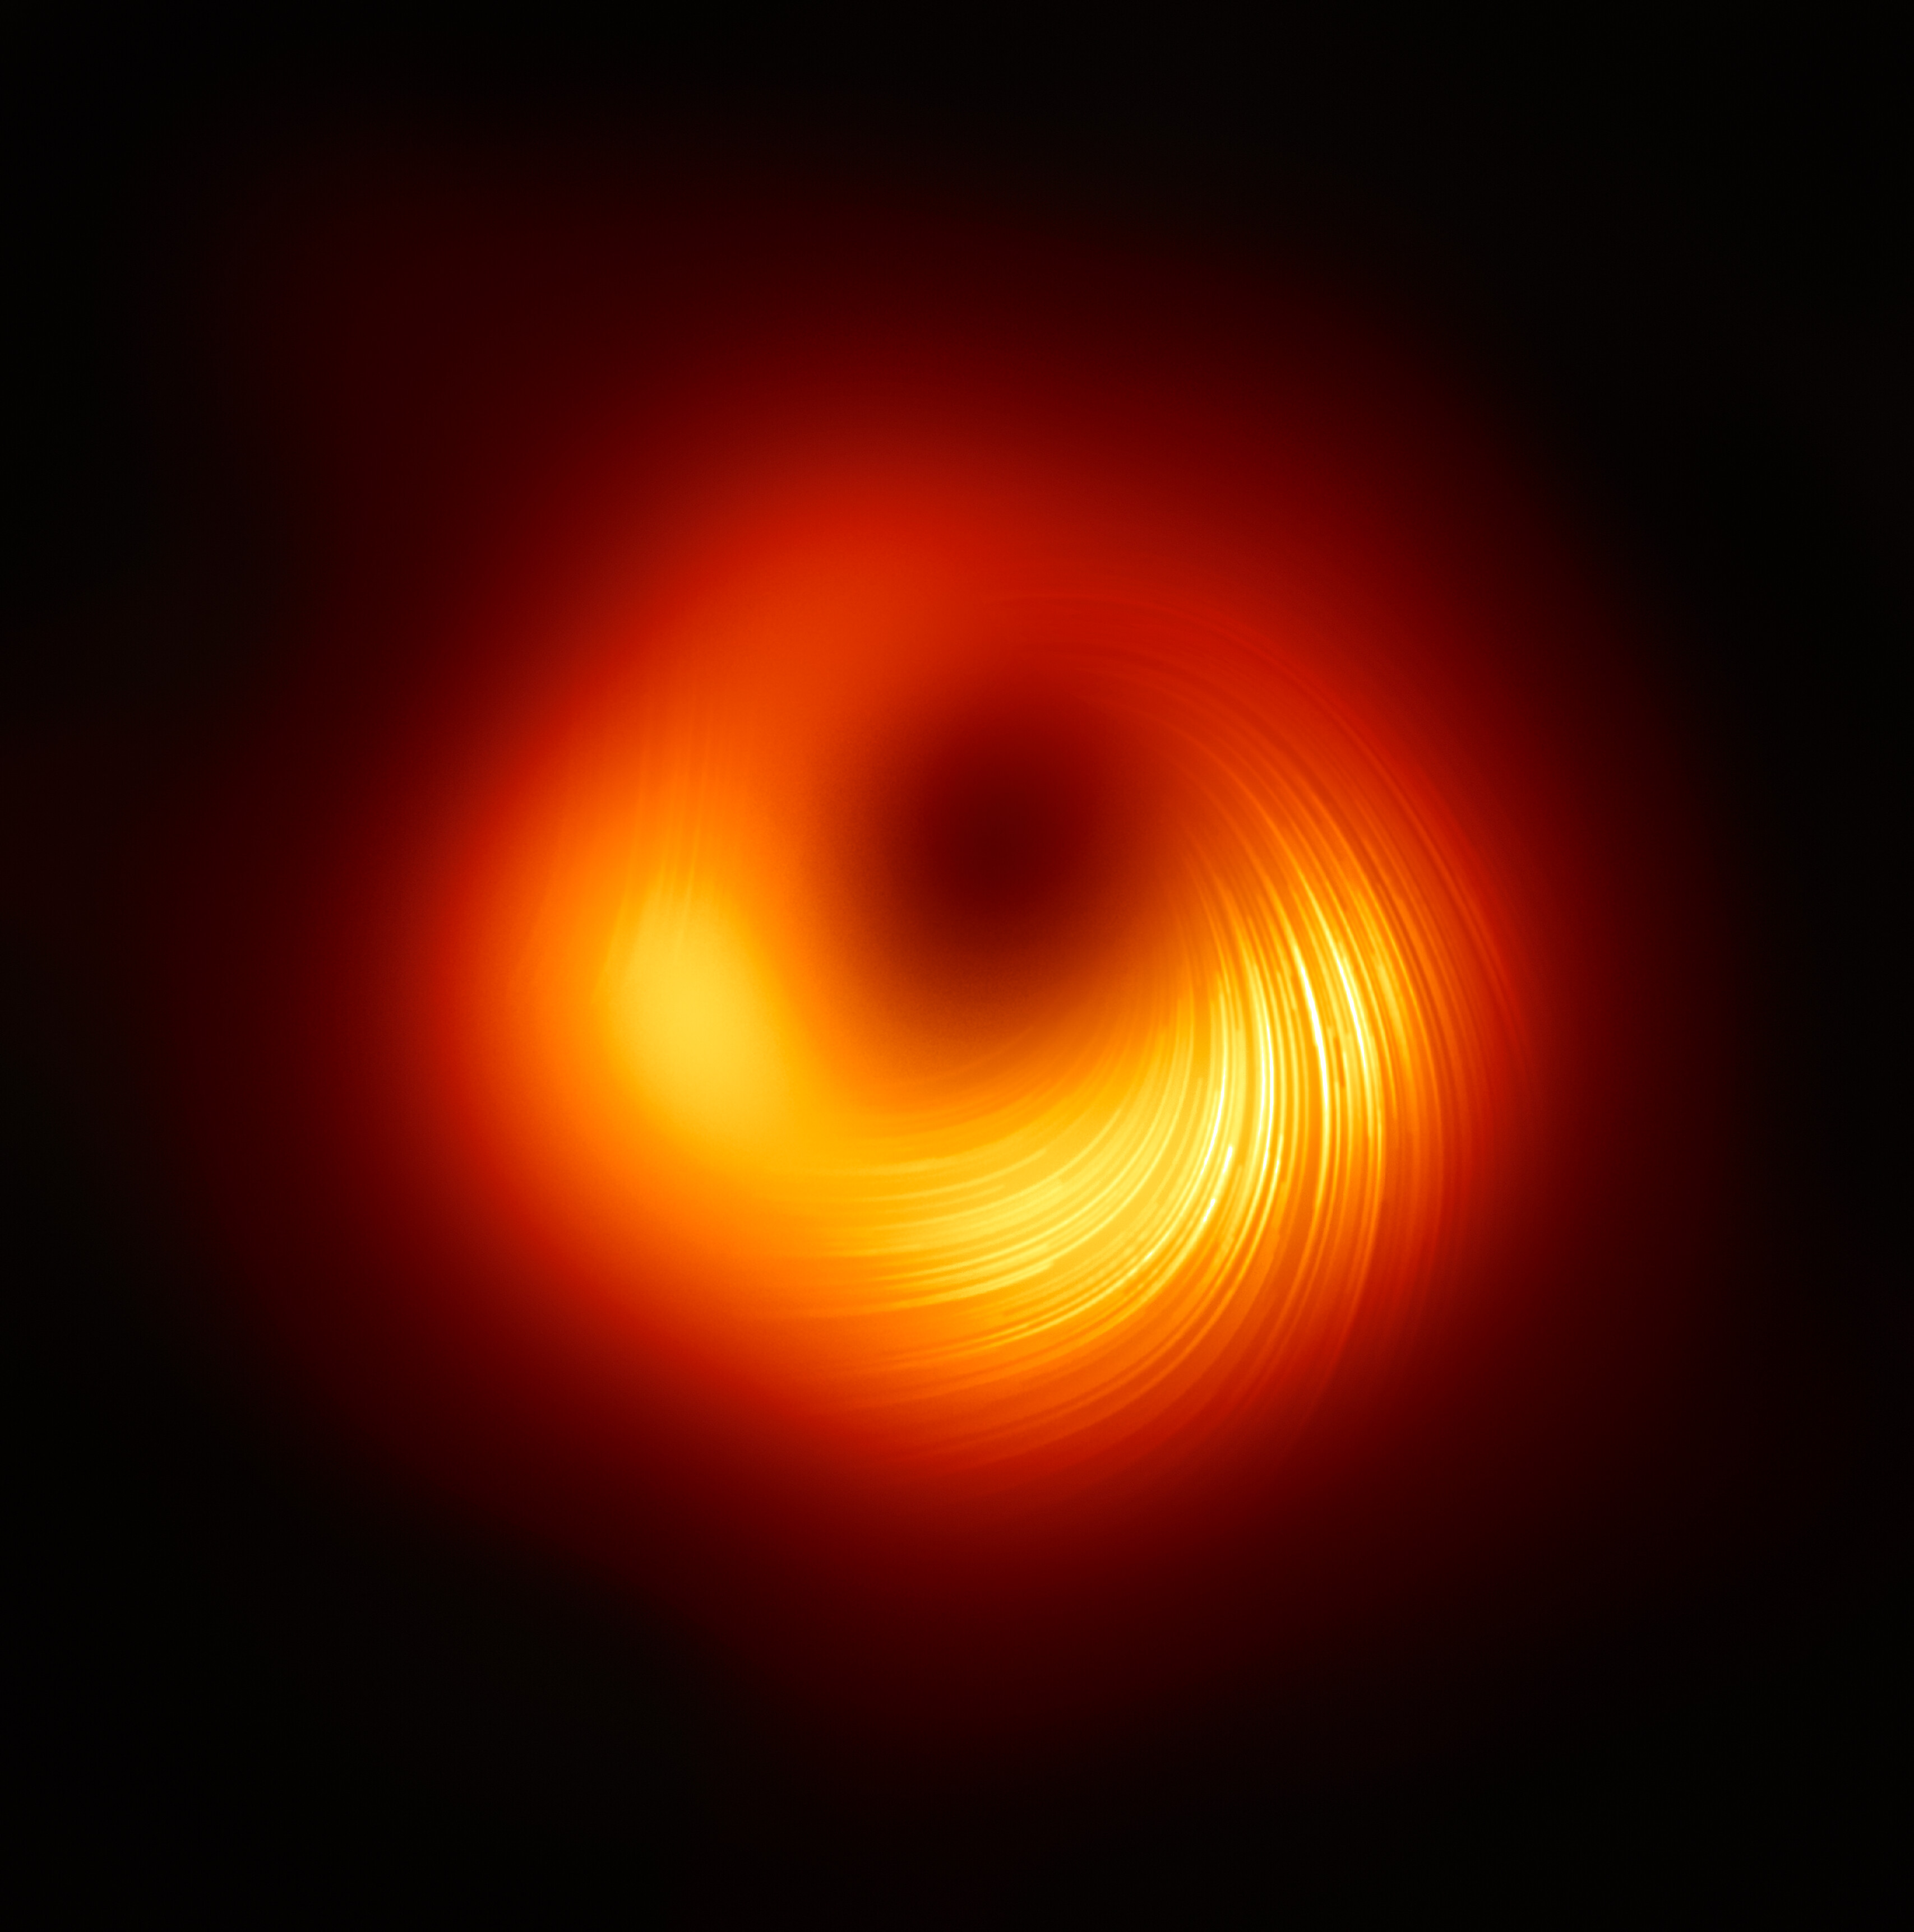
\includegraphics[width=0.7\linewidth]{c96e01c894dab21d52bb0bd6565f0331.jpg}}
	\caption{Восстановленная фотография тени чёрной дыры.}
	\label{fig:vosstanovlennaya_fotografiya_chyornoj_dyry}
\end{figure}
Обрантим внимание на парамет <<[H]>> окружения \textsc{figure}. Этот параметр определяет место рисунка в тексте: разрешить алгоритмам ТеХа принять решение исходя из заполненности страницы [h] "хотелось бы картинку здесь"; настойчиво просить разместить после текста [h!] "очень хочу картинку здесь"; и ударить кулаком по столу "--- картинку тут и точка [H] "ХОЧУ картинку здесь и баста"; а с прибавлением буквы "p" мы заставляем поместить ЛаТеХ картинку отдельно на страницу так [pH] "--- см. \url{https://mydebianblog.blogspot.com/2008/12/latex_15.html}.

Теперь попытаемся построить рисунок (графики) с помощью \texttt{gnuplot} и одноимённого с ним окружения из пакета \textsc{gnuplottex}.
%\begin{Verbatim}[fontfamily = courier, tabsize = 3, numbers = left, gobble=1]
\lstset{language = Gnuplot, frame = none, tabsize = 3, numbers = left, numbersep = 6pt, gobble=1}%
\begin{lstlisting}
	\begin{figure}[h]%
		\centering%
		\begin{gnuplot}[terminal = epslatex, terminaloptions = {color dashed}]
			set key box top left
			set key width 4
			set sample 1000
			set xr [-5:5]
			set yr [-1:1]
			set xlabel '$x$-label'
			set ylabel '$y$-label'
			plot sin(x) w l lc 1 t '$\sin(x)$',\
			cos(x) w l lc 2 t '$\cos(x)$',\
			tan(x) w l lc 3 t '$\tan(x)$',\
			tanh(x) w l lc 4 t '$5\tanh(x)$'
		\end{gnuplot}
		\caption{This is a simple example using the latex-terminal.}%
		\label{fig:latex}%
	\end{figure}
\end{lstlisting}

%\begin{gnuplot}[terminal=pdf,terminaloptions=font ”,10” linewidth 3]
\begin{figure}[h]%
	\centering%
	\begin{gnuplot}[terminal = epslatex, terminaloptions = {color dashed}]
		set key box top left
		set key width 4
		set sample 1000
		set xr [-5:5]
		set yr [-1:1]
		set xlabel '$x$-label'
		set ylabel '$y$-label'
		plot sin(x) w l lc 1 t '$\sin(x)$',\
		cos(x) w l lc 2 t '$\cos(x)$',\
		tan(x) w l lc 3 t '$\tan(x)$',\
		tanh(x) w l lc 4 t '$5\tanh(x)$'
	\end{gnuplot}
	\caption{Пример работы \texttt{gnuplot}.}%
	\label{fig:primer_raboty_gnuplot}%
\end{figure}%
Для автоматического построения графика средствами \texttt{gnuplot} необходимо также добавить ключ \texttt{shell escape} в команде компиляции tex-файла: \verb|pdflatex --synctex=1 --shell-escape default|.

Расмотрим пример построения блок-схем с использованием пакета \textsc{tikz} с подключёнными библиотеками \textsl{arrows} и \textsl{shapes} перечислив их в \{~\}\nobreak-скобках команды \textsc{usetikzlibrary}, для построения графов же "--- \textsl{graphs}. Описание блок схем помещаются в тело окружения \textsc{tikzpicture}: узлы вводятся и описываюся командой \textsc{node}, а пути - командой \textsc{path}. Пусть нам нужно описать алгоритм программы \texttt{testx3p}, написаной на фортране (см.~директорию~\textsl{app}):

%\VerbatimInput[frame = none, label = {Листинг программы \texttt{testx3p}}, fontfamily = courier, tabsize = 3, numbers = left, numbersep = 6pt]{src/testx3p.f08}%
\lstset{language = [08]Fortran, frame = none, name = {Листинг программы \texttt{testx3p}}, tabsize = 3, numbers = left, numbersep = 6pt}\lstinputlisting{src/testx3p.f08}%

Для удобства опишем несколько \textsl{tikz}\nobreak-стилей согласно \textbf{ГОСТ 19.701-90 <<Схемы алгоритмов программ, данных и систем>>} "---~см.~\cite{mkrtumyan:tech:2010:01}, с помощью команды \textsc{tikzset}:

\verb|\tikzset{<имя_стиля>/.style = {<параметры_стиля>}}|.

Используемые стили см.~в исходном tex\nobreak-файле настоящей статьи.

Таким образом,

\tikzset{terminator/.style = {% терминатор - начало или конец любой функции/подпрограммы
		rectangle, draw, text centered, rounded corners, minimum height = 2em
	}
}
\tikzset{operator/.style = {% блок выполнения операций над данными
		rectangle, draw, text centered, minimum height = 2em
	}
}
\tikzset{decision/.style = {% блок оператора ветвления
		diamond, draw, text centered, minimum height = 2em
	}
}
\tikzset{data/.style = {% блок ввода-ввывода данных
		trapezium, draw, text centered, trapezium left angle = 60,
		trapezium right angle = 120, minimum height = 2em
	}
}
\tikzset{link/.style = {% связь
		draw, -latex'
	}
}
\tikzset{connector/.style = {% соединитель, есть штатный стиль "state"
		circle, draw, text centered, minimum height = 2em
	}
}
\tikzset{function/.style = {% блок вызова внешней функции
		rectangle split, rectangle split horizontal,
		rectangle split parts = 3,
		draw, text centered,
		minimum width = 5em,
		minimum height = 2em,
		outer sep = 0
	}
}
\tikzset{subroutine/.style = {% блок вызова внешней подпрограммы
		rectangle split, rectangle split horizontal,
		rectangle split parts = 3,
		draw, text centered,
		minimum width = 5em,
		minimum height = 2em,
		outer sep = 0
	}
}
\tikzset{procedure/.style = {% блок вызова внешней процедуры
		rectangle split, rectangle split horizontal,
		rectangle split parts = 3,
		draw, text centered,
		minimum width = 5em,
		minimum height = 2em,
		outer sep = 0
	}
}
\tikzset{loop/.style = {% блок-начало цикла с условием
		chamfered rectangle,
		chamfered rectangle corners={
			north west, north east
		},
		draw, text centered,
		minimum width = 5em,
		minimum height = 2em,
		outer sep = 0
	}
}
\tikzset{endloop/.style = {% блок-конец цикла с условием
		chamfered rectangle,
		chamfered rectangle corners={
			south west, south east
		},
		draw, text centered,
		minimum width = 5em,
		minimum height = 2em,
		outer sep = 0
	}
}
\tikzset{counterloop/.style = {% блок цикла со счётчиком
		chamfered rectangle,
		chamfered rectangle xsep = 2cm,
		draw, text centered,
		minimum width = 5em,
		minimum height = 2em,
		outer sep = 0
	}
}
\tikzset{preparation/.style = {% блок подготовки данных
		rectangle split, rectangle split horizontal,
		rectangle split parts = 3,
		draw, text centered,
		minimum width = 5em,
		minimum height = 2em,
		outer sep = 0
	}
}

\begin{tikzpicture}[node distance = 1.7cm, auto]
	\node [terminator] at (0,0) (start) {\textbf{Начало}};
	\node [data, below of = start, node distance=1.5cm] (input) {$x$, $y$, $i$, $j$, $n$, массив $p$};
	\node [operator, below of = input, node distance=1.5cm] (openfile) {Открыть файл \textsl{data.res}, id = n};
	\node [operator, below of = openfile, node distance=1.5cm] (output1) {Записать {\tt $p[]$} в файл \textsl{data.res}};
	\node [loop, below of = output1, node distance=1.5cm] (loop) {Главный цикл расчёта \\ $i = \overline{0,20}$};
	\node [operator, below of = loop, node distance=1.5cm] (calculation) {$x = -1 + i 0,1$};
	\node [operator, below of = calculation, node distance=1.5cm] (output2) {Записать {\tt $x$, $(x + p_{j})^{3}$ $\forall j = \overline{-4,4}$} в файл \textsl{data.res}};
	\node [endloop, below of = output2, node distance=1.5cm] (endloop) {Главный цикл расчёта};
	\node [terminator, below of = endloop, node distance=1.5cm] (end) {\textbf{Конец}};
	\path [-] (start) edge (input);
	\path [-] (input) edge (openfile);
	\path [-] (openfile) edge (output1);
	\path [-] (output1) edge (loop);
	\path [-] (loop) edge (calculation);
	\path [-] (calculation) edge (output2);
	\path [-] (output2) edge (endloop);
	\path [-] (endloop) edge (end);
\end{tikzpicture}

Для случая блок\nobreak-схемы вызова внешней подпрограммы (см.~\url{https://pro-prof.com/archives/1462}) мы используем следующий стиль:

%\lstset{language = [LaTeX]TeX, name = {Пример стиля \texttt{tikz}}, frame = none, tabsize = 3, numbers = left, numbersep = 6pt, gobble=1}%
%\begin{lstlisting}
\begin{Verbatim}[fontfamily = courier, tabsize = 3, numbers = left, gobble=1]
	\tikzset{subroutine/.style = {% блок вызова внешней подпрограммы
			rectangle split, rectangle split horizontal,
			rectangle split parts = 3,
			draw, text centered,
			minimum width = 5em,
			minimum height = 2em,
			outer sep = 0
		}
	}%
	\begin{tikzpicture}
		\node [subroutine] at (0,0) (subroutine) {\nodepart{two}\textbf{Подпрограмма}};
	\end{tikzpicture}%
\end{Verbatim}
%\end{lstlisting}

\begin{tikzpicture}
	\node [subroutine] at (0,0) (subroutine) {\nodepart{two}\textbf{Подпрограмма}};
\end{tikzpicture}

Обратите внимание, что для корректной работы перед содержимым блока в \textsc{node} необходимо прописать \verb|\nodepart{two}|.

Описание tikz\nobreak-стилей (да и других) рекомендуется сохранять в отдельном tex\nobreak-файле и подключать его в преамбуле, или в начале тело документа с помощью команды \textsc{input}.

Построим график из данных расчёта программы \texttt{testx3p}.


Результаты расчёта записываются программой в файл \textsl{testx3p.res} в поддиректорию \textsl{data}. После небольшой обработки содержимомго файла под нужды пакета \textsc{tabularray} и записи результата в файл \textsl{tbl1.tex} в поддиректорию \textsl{tables} мы можем представить эти данные в табличной виде:

%{{{ Horrible hack

\ExplSyntaxOn
% read the file content
\file_get:nnN {tables/tbl1} {\ExplSyntaxOff} \tblone
\ExplSyntaxOff

%}}}

\begin{longtblr}[
% 	theme = fancy,
	caption = {Результаты расчёта программы \texttt{testx3p}.},
	entry = {Расчёта программы \texttt{testx3p}.},
	label = {tblr:rezultaty_raschyota_programmy_testx3p},
% 	note{a} = {Это первая сноска.},
% 	note{$\dag$} = {Это вторая длинная сноска.},
% 	remark{Примечание} = {Некоторые общие примечания.},
% 	remark{Источник} = {Сделано силами авторов.},
	baseline = m,
	expand = \expandafter,
]{
	rows = {c},
	columns = {r},
	row{odd} = {bg = azure8},
	row{1} = {m,bg = azure3, fg = white, font = \sffamily},
	row{1}{1} = {c},
	rowhead = 1,
	rowfoot = 0,
	width=\textwidth,
	hlines,
	vlines,
}
	%	\diagbox{x}{p} & -0,90 & -0,50 & -0,30 & -0,10 & 0,00 & 0,10 & 0,30 & 0,50 & 0,90 \\
	-1,00 & -6,86 & -3,38 & -2,20 & -1,33 & -1,00 & -0,73 & -0,34 & -0,12 & -0,00 \\
	-0,90 & -5,83 & -2,74 & -1,73 & -1,00 & -0,73 & -0,51 & -0,22 & -0,06 & 0,00 \\
	-0,80 & -4,91 & -2,20 & -1,33 & -0,73 & -0,51 & -0,34 & -0,12 & -0,03 & 0,00 \\
	-0,70 & -4,10 & -1,73 & -1,00 & -0,51 & -0,34 & -0,22 & -0,06 & -0,01 & 0,01 \\
	-0,60 & -3,38 & -1,33 & -0,73 & -0,34 & -0,22 & -0,12 & -0,03 & -0,00 & 0,03 \\
	-0,50 & -2,74 & -1,00 & -0,51 & -0,22 & -0,12 & -0,06 & -0,01 & 0,00 & 0,06 \\
	-0,40 & -2,20 & -0,73 & -0,34 & -0,12 & -0,06 & -0,03 & -0,00 & 0,00 & 0,12 \\
	-0,30 & -1,73 & -0,51 & -0,22 & -0,06 & -0,03 & -0,01 & 0,00 & 0,01 & 0,22 \\
	-0,20 & -1,33 & -0,34 & -0,12 & -0,03 & -0,01 & -0,00 & 0,00 & 0,03 & 0,34 \\
	-0,10 & -1,00 & -0,22 & -0,06 & -0,01 & -0,00 & 0,00 & 0,01 & 0,06 & 0,51 \\
	0,00 & -0,73 & -0,12 & -0,03 & -0,00 & 0,00 & 0,00 & 0,03 & 0,12 & 0,73 \\
	0,10 & -0,51 & -0,06 & -0,01 & 0,00 & 0,00 & 0,01 & 0,06 & 0,22 & 1,00 \\
	0,20 & -0,34 & -0,03 & -0,00 & 0,00 & 0,01 & 0,03 & 0,13 & 0,34 & 1,33 \\
	0,30 & -0,22 & -0,01 & 0,00 & 0,01 & 0,03 & 0,06 & 0,22 & 0,51 & 1,73 \\
	0,40 & -0,12 & -0,00 & 0,00 & 0,03 & 0,06 & 0,12 & 0,34 & 0,73 & 2,20 \\
	0,50 & -0,06 & 0,00 & 0,01 & 0,06 & 0,12 & 0,22 & 0,51 & 1,00 & 2,74 \\
	0,60 & -0,03 & 0,00 & 0,03 & 0,12 & 0,22 & 0,34 & 0,73 & 1,33 & 3,38 \\
	0,70 & -0,01 & 0,01 & 0,06 & 0,22 & 0,34 & 0,51 & 1,00 & 1,73 & 4,10 \\
	0,80 & -0,00 & 0,03 & 0,13 & 0,34 & 0,51 & 0,73 & 1,33 & 2,20 & 4,91 \\
	0,90 & 0,00 & 0,06 & 0,22 & 0,51 & 0,73 & 1,00 & 1,73 & 2,74 & 5,83 \\
	1,00 & 0,00 & 0,12 & 0,34 & 0,73 & 1,00 & 1,33 & 2,20 & 3,38 & 6,86 \\
 % не работает!
	\expandafter\empty\tblone

\end{longtblr}

Путь к исходному файлу с данными \textsl{testx3p.res} мы пропишем в сам скрипт gnuplot для построения графиков, который сохраним в отдельном файле, а затем подключим его в \TeX\ документ с помощью команды \textsc{gnuplotloadfile}, например \\ \verb|\gnuplotloadfile[<параметры>]{scr/testx3p1.gp}|. Тогда
\begin{figure}[h]%
	\centering%
	\gnuplotloadfile[terminal = epslatex, terminaloptions = {color dashed}]{scr/testx3p1.gp}
	\caption{Семейство кривых функции $f(x) = (x + p)^{3}$.}%
	\label{fig:semejstvo_krivyx_funkcii_fx}%
\end{figure}%

Подробнее этот пример программы на \textsl{фортране} и взаимодействия с \texttt{gnuplot} см.~\cite{shnejvajs:book:2016:01}.



%заключение
\section{Заключение}
\label{sec:conclusion}


В заключении отметим, что данное руководство в большей степени пример; для полнового введения лучше обратиться к справичникам и к указанной литературе. По-началу поттребуется много практики для освоения языка программирования \LaTeX. Вместе с тем \texttt{gnuplot} был выбран из-за простоти в его освоении, и хорошей связки с \LaTeX. Тем не менее, можно строить графики средствами самого \LaTeX а, а именно при помощи того же пакета \textsc{tikz}, использованного для построения блок-схем. Однако рекомендуется сначала освоиться с \textsl{базовым} \LaTeX ом.



% \section*{\refname}
% \addtocontents{toc}{section}{Список литературы}
\label{sec:references}


%\bibliographystyle{gost7184}
\bibliography{bib/main}



\newpage
\section{Приложение}
\label{sec:application}


%{{{ Horrible hack

\ExplSyntaxOn
% read the file content
\file_get:nnN {tables/tbl2} {\ExplSyntaxOff} \tbltwo
\ExplSyntaxOff

%}}}

\begin{longtblr}[
% 	theme = fancy,
	caption = {Результаты моделирования движения частицы.},
	entry = {Баллистическое движение частицы.},
	label = {tblr:rezultaty_modelirovaniya_dvizheniya_chasticy},
% 	note{a} = {Это первая сноска.},
% 	note{$\dag$} = {Это вторая длинная сноска.},
% 	remark{Примечание} = {Некоторые общие примечания.},
% 	remark{Источник} = {Сделано силами авторов.},
	baseline = m,
	expand=\expandafter,
]{
	rows = {c},
	columns = {r},
	row{odd} = {bg = azure8},
	row{1-2} = {c, bg = azure3, fg = white, font = \sffamily},
	rowhead = 2,
	rowfoot = 0,
	width=\textwidth,
	hlines,
	vlines,
}
% 	\hline
		\SetCell[r = 2]{c} {Время \\ $t$, с}
			& \SetCell[c = 2]{c} {Координаты}
				&	& \SetCell[c = 2]{c} {Скорость} & \\
% 	\hline
			& $x$, м & $y$, м & $v_{x}$, м/с & $v_{y}$, м/с \\
% 	\hline
	%	\diagbox{x}{p} & -0,90 & -0,50 & -0,30 & -0,10 & 0,00 & 0,10 & 0,30 & 0,50 & 0,90 \\
	-1,00 & -6,86 & -3,38 & -2,20 & -1,33 & -1,00 & -0,73 & -0,34 & -0,12 & -0,00 \\
	-0,90 & -5,83 & -2,74 & -1,73 & -1,00 & -0,73 & -0,51 & -0,22 & -0,06 & 0,00 \\
	-0,80 & -4,91 & -2,20 & -1,33 & -0,73 & -0,51 & -0,34 & -0,12 & -0,03 & 0,00 \\
	-0,70 & -4,10 & -1,73 & -1,00 & -0,51 & -0,34 & -0,22 & -0,06 & -0,01 & 0,01 \\
	-0,60 & -3,38 & -1,33 & -0,73 & -0,34 & -0,22 & -0,12 & -0,03 & -0,00 & 0,03 \\
	-0,50 & -2,74 & -1,00 & -0,51 & -0,22 & -0,12 & -0,06 & -0,01 & 0,00 & 0,06 \\
	-0,40 & -2,20 & -0,73 & -0,34 & -0,12 & -0,06 & -0,03 & -0,00 & 0,00 & 0,12 \\
	-0,30 & -1,73 & -0,51 & -0,22 & -0,06 & -0,03 & -0,01 & 0,00 & 0,01 & 0,22 \\
	-0,20 & -1,33 & -0,34 & -0,12 & -0,03 & -0,01 & -0,00 & 0,00 & 0,03 & 0,34 \\
	-0,10 & -1,00 & -0,22 & -0,06 & -0,01 & -0,00 & 0,00 & 0,01 & 0,06 & 0,51 \\
	0,00 & -0,73 & -0,12 & -0,03 & -0,00 & 0,00 & 0,00 & 0,03 & 0,12 & 0,73 \\
	0,10 & -0,51 & -0,06 & -0,01 & 0,00 & 0,00 & 0,01 & 0,06 & 0,22 & 1,00 \\
	0,20 & -0,34 & -0,03 & -0,00 & 0,00 & 0,01 & 0,03 & 0,13 & 0,34 & 1,33 \\
	0,30 & -0,22 & -0,01 & 0,00 & 0,01 & 0,03 & 0,06 & 0,22 & 0,51 & 1,73 \\
	0,40 & -0,12 & -0,00 & 0,00 & 0,03 & 0,06 & 0,12 & 0,34 & 0,73 & 2,20 \\
	0,50 & -0,06 & 0,00 & 0,01 & 0,06 & 0,12 & 0,22 & 0,51 & 1,00 & 2,74 \\
	0,60 & -0,03 & 0,00 & 0,03 & 0,12 & 0,22 & 0,34 & 0,73 & 1,33 & 3,38 \\
	0,70 & -0,01 & 0,01 & 0,06 & 0,22 & 0,34 & 0,51 & 1,00 & 1,73 & 4,10 \\
	0,80 & -0,00 & 0,03 & 0,13 & 0,34 & 0,51 & 0,73 & 1,33 & 2,20 & 4,91 \\
	0,90 & 0,00 & 0,06 & 0,22 & 0,51 & 0,73 & 1,00 & 1,73 & 2,74 & 5,83 \\
	1,00 & 0,00 & 0,12 & 0,34 & 0,73 & 1,00 & 1,33 & 2,20 & 3,38 & 6,86 \\
 % не работает!
	\expandafter\empty\tbltwo

\end{longtblr}



\end{document}


